% !TeX program = lualatex
%======================================================================%
% Accessible LaTeX Template (PDF/UA-2): Worked Example
% Developed and maintained by Gerry Pedraza and Christine Roach,
% Engineering Studio for Advanced Instruction and Learning (eSAIL),
% Texas A&M University
% https://github.com/gerrypedraza/accessibility
% License: MIT. Suggestions or problems: open an issue on the repository.
%
% Based on the LaTeX Tagging Project by the LaTeX Project Team:
%   Usage instructions: https://tagging-project.latex-project.org/documentation/usage-instructions
%   Package compatibility: https://latex3.github.io/tagging-project/tagging-status/
%
% REQUIREMENTS
%   - LaTeX kernel 2025-11-01 or newer (tested with 2026-06-01)
%   - Overleaf: Menu > Settings > TeX Live version > Rolling TeX Live
%   - Compiler: LuaLaTeX (required for automatic MathML)
% Goal: output that works well with NVDA + MathCAT.
%======================================================================%

% --- 1. METADATA AND PDF STANDARD (MUST come before \documentclass) ---

% ===== MODE A: STANDARD (recommended) - PDF 2.0, PDF/UA-2, MathML =====
\DocumentMetadata{
  lang        = en-US,
  pdfversion  = 2.0,
  pdfstandard = ua-2,
  tagging     = on,        % loads all tagging modules (math, tables, lists...)
  check-tagging-status,    % log reports each package's tagging compatibility
  tagging-setup = {
    % mathml-SE: MathML as structure elements in the tag tree
    % mathml-AF: MathML as an associated (embedded) file
    % Readers differ in which they support; we include both.
    math/setup        = {mathml-SE, mathml-AF},
    % Experimental: tags verbatim as code so punctuation ( ) { } / is spoken
    extra-modules     = {verbatim-mo},
    % First table row = header (TH). Override per table with
    % \tagpdfsetup{table/header-rows={...}}; for layout-only tables use
    % \tagpdfsetup{table/tagging=presentation}
    table/header-rows = 1
  }
}

% ===== MODE B: COMPATIBILITY - PDF 1.7, PDF/UA-1, alt-text math ======
% For platforms/checkers that only evaluate UA-1 (e.g., to satisfy Ally).
% Equations have NO MathML: screen readers get alt text only, with no
% term-by-term navigation. Comment out Mode A and uncomment below.
%\DocumentMetadata{
%  lang        = en-US,
%  pdfversion  = 1.7,
%  pdfstandard = ua-1,
%  tagging     = on,
%  check-tagging-status,
%  tagging-setup = {
%    extra-modules     = {verbatim-mo},
%    table/header-rows = 1
%  }
%}

\documentclass[11pt]{article}

% --- 2. PAGE LAYOUT ---------------------------------------------------
\usepackage[letterpaper, margin=1in]{geometry}

% --- 3. MATH (order matters) ------------------------------------------
\usepackage{amsmath}       % environments: align, cases, \text, etc.
\usepackage{unicode-math}  % load AFTER amsmath. Unicode math fonts enable
                           % MathML generation. Loads fontspec.
                           % DO NOT also load amssymb or amsfonts.
% Optional styling: IEEE-like Times fonts (text and matching math).
% Must come after unicode-math. Comment out both lines for the defaults.
\setmainfont{STIX Two Text}
\setmathfont{STIX Two Math}

% --- 4. GRAPHICS, TABLES, CAPTIONS ------------------------------------
\usepackage{graphicx}      % every image needs one of:
                           %   \includegraphics[alt={...}]{file}
                           %   \includegraphics[artifact]{file} (decorative)
                           % alt text = educational purpose, not appearance
\usepackage{booktabs}      % compatible with tagging
\usepackage{caption}
\usepackage{float}         % provides the [H] placement specifier

% IEEE-like caption settings
\renewcommand{\tablename}{TABLE}
\renewcommand{\thetable}{\Roman{table}}
\captionsetup[table]{%
  labelfont=bf,
  textfont=normalfont,
  labelsep=period
}
\captionsetup[figure]{%
  labelfont=bf,
  textfont=normalfont,
  labelsep=period,
  name=Fig.
}

% --- 5. LINKS AND PDF METADATA (load last) ----------------------------
\usepackage{hyperref}
\hypersetup{
  pdftitle={Accessibility Recommendations for LaTeX Documents},  % required by PDF/UA
  pdfauthor={eSAIL @ TAMU - Accessibility Team},
  pdfsubject={Accessible LaTeX Recommendations (PDF/UA-2)},
  pdfkeywords={LaTeX, accessibility, PDF/UA-2, NVDA, MathML},
  pdfdisplaydoctitle=true
}

% --- DO NOT USE -------------------------------------------------------
% \usepackage{accessibility}  % deprecated (2020), targets PDF 1.5/1.6;
%                             % replaced by \DocumentMetadata tagging
% \usepackage{amssymb}        % redundant/conflicts with unicode-math
% XeLaTeX or pdfLaTeX         % no automatic MathML

% --- 6. TITLE / AUTHOR / DATE -----------------------------------------
\title{Accessibility Recommendations for LaTeX Documents}
\author{eSAIL @ TAMU - Instructional Design + Accessibility Team}
\date{October 2026}

% Anchor command for a precise jump-back point
\newcommand{\returnanchor}[1]{\phantomsection\label{#1}}

% --- 7. BUILD INFORMATION (optional) ----------------------------------
% \BuildInfo prints the compile setup: engine and TeX Live version, LaTeX
% release, whether tagging is on, PDF version, unicode-math version, main
% font, and date. Useful for checking a setup or reporting a problem.
\makeatletter
\ExplSyntaxOn
\NewDocumentCommand{\BuildInfo}{}{
  \begin{itemize}
    \item \textbf{Engine:}~
      \cs_if_exist:NTF \directlua
        { \directlua{tex.sprint(-2, status.banner)} }
        { Not~LuaLaTeX.~Switch~the~compiler~to~LuaLaTeX~for~automatic~MathML. }
    \item \textbf{LaTeX~release:}~\fmtversion
      \tl_if_eq:NnF \patch@level { 0 } { ~(patch~level~\patch@level) }
    \item \textbf{Tagging:}~
      \cs_if_exist:NTF \tag_if_active:TF
        { \tag_if_active:TF { on } { off } }
        { not~available~(LaTeX~release~too~old) }
    \item \textbf{PDF~version:}~
      \cs_if_exist:NTF \pdf_version: { \pdf_version: } { unknown }
    \item \textbf{unicode-math:}~
      \cs_if_exist:cTF { ver@unicode-math.sty }
        { \use:c { ver@unicode-math.sty } } { not~loaded }
    \item \textbf{Main~font:}~\fontname\font
    \item \textbf{Compiled~on:}~\today
  \end{itemize}
}
\ExplSyntaxOff
\makeatother

\begin{document}
\sloppy % Relaxes line-breaking to prevent overfull hbox warnings

\maketitle

%======================================================================%
% DISCLAIMER / INTRODUCTION
%======================================================================%
\section{Disclaimer and Context}

These accessibility recommendations are based on the knowledge gathered by the eSAIL team at Texas A\&M and the work of the LaTeX Tagging Project [1], [2]. They represent current best practices for creating PDF/UA-2 documents with LuaLaTeX. Tagging support in LaTeX is under active development, so check the project's documentation for changes.

\textbf{Requirements:} This document requires the LaTeX release of 2025-11-01 or newer and must be compiled with LuaLaTeX. On Overleaf, select \emph{Rolling TeX Live} in the project settings; the default TeX Live version is too old for these settings.

\textbf{Instructional Note on Metadata:} In the source code of this document, the \texttt{\textbackslash DocumentMetadata} command appears before \texttt{\textbackslash documentclass}. Its \texttt{tagging=on} key replaces the older \texttt{testphase} setups and loads all the code needed to tag paragraphs, lists, tables, and math [1]. The \texttt{check-tagging-status} key writes a report to the log file listing whether each package you load is compatible with tagging.

\subsection{Build Information}
The list below is generated when the document compiles, using the \verb|\BuildInfo| command defined in the preamble. Use it to confirm the requirements above: the engine should be LuaLaTeX, the LaTeX release 2025-11-01 or newer, tagging on, and the PDF version 2.0.
\BuildInfo

%======================================================================%
% SECTION 1: BASIC STRUCTURE
%======================================================================%
\section{Basic Document Structure and Headings}

\subsection{Template Style}
This example uses IEEE-style conventions for captions and the Times-like STIX Two fonts for text and math. Under LuaLaTeX these are OpenType fonts that embed as Unicode, so text and math can be extracted and read aloud correctly.

\subsection{Sample Paragraph and Tagging}
Because the \verb|\section| and \verb|\subsection| commands are used, the PDF tagging system maps these lines to semantic heading tags. Screen readers use these headings to navigate the document.

\subsection{Lists (Semantic Bullets and Steps)}
We use the standard \verb|itemize| and \verb|enumerate| environments. The \texttt{tagging=on} setting automatically converts these into \texttt{L} (List), \texttt{LI} (List Item), \texttt{Lbl} (Label), and \texttt{LBody} (List Body) tags, which screen readers need to announce lists correctly.

Unordered list:
\begin{itemize}
  \item Use \verb|\begin{itemize}| for bullet lists.
  \item Screen readers announce lists and list items.
\end{itemize}

Ordered list:
\begin{enumerate}
  \item First step in the process.
  \item Second step in the process.
\end{enumerate}

\subsection{Links with Meaningful Link Text}
For example, visit the \href{https://www.tamu.edu}{Texas A\&M University website} instead of writing out the raw URL.

%======================================================================%
% SECTION 2: DATA PRESENTATION
%======================================================================%
\section{Data Presentation (Accessible Tables and Figures)}

\subsection{Why We Use Global Header Settings}
In the preamble, we set \texttt{table/header-rows=1}. This tells the compiler to tag the first row of \emph{every} table as a header row (\texttt{TH}). Without header cells, screen readers cannot associate the data in row 5 with the label in row 1.

Because this is a global default, override it for tables that are different: use \verb|\tagpdfsetup{table/header-rows={1,2}}| before a table with two header rows, or \verb|\tagpdfsetup{table/tagging=presentation}| before a table used only for layout.

\begin{table}[htbp]
    \caption{Selected Material Properties for Common Engineering Elements}
    \label{tab:material-properties}
    \centering
    \small
    % Two header rows (names, then units): override the global default
    % here, inside the table environment, so it applies to this table.
    \tagpdfsetup{table/header-rows={1,2}}
    \begin{tabular}{l c c c c}
        \toprule
        \textbf{Element} &
        \textbf{Density} &
        \textbf{Melting point} &
        \textbf{Thermal conductivity} &
        \textbf{Young's modulus} \\
         &
        (g/cm\textsuperscript{3}) &
        (°C) &
        (W/m·K) &
        (GPa) \\
        \midrule
        Aluminum (Al) & 2.70  & 660  & 237  & 70  \\
        Steel (Fe)    & 7.87  & 1538 & 80.4 & 210 \\
        Copper (Cu)   & 8.96  & 1085 & 401  & 110 \\
        Titanium (Ti) & 4.51  & 1668 & 21.9 & 116 \\
        Tungsten (W)  & 19.25 & 3422 & 173  & 411 \\
        \bottomrule
    \end{tabular}
\end{table}

\subsection{Example: Data Presentation Figure}
This figure demonstrates the ``long description'' pattern: short alt text that states the figure's purpose, plus a caption link to a full description in the appendix.

Alt text should describe what the reader is meant to learn from the figure, not only what it looks like.

\begin{figure}[htbp]
    \centering
    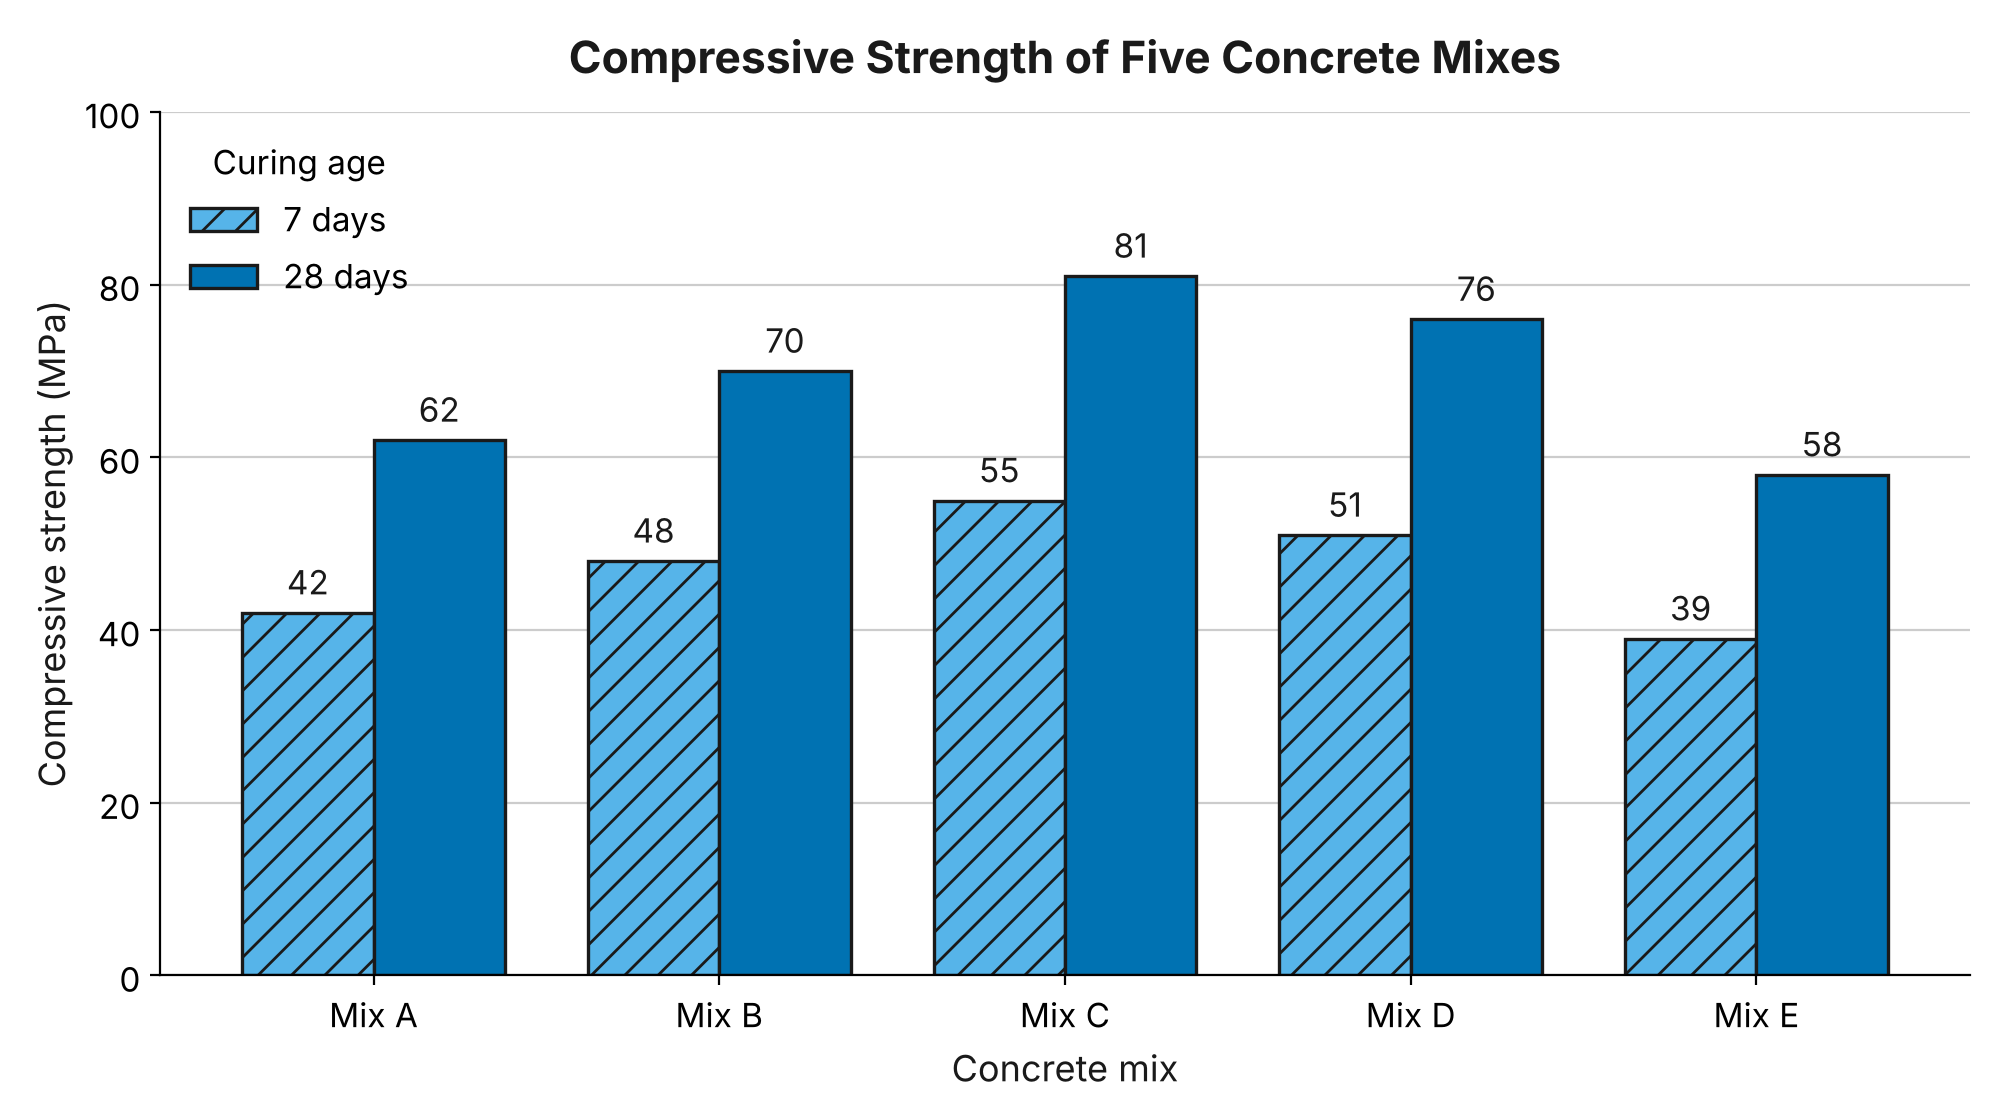
\includegraphics[
      width=0.9\linewidth,
      alt={Bar chart of concrete strength at 7 and 28 days. Mix C is strongest; all mixes gain strength. Details in Appendix A.}
    ]{images/data-presentation-image.png}
    \caption{Compressive Strength of Five Concrete Mixes, illustrative data (\hyperref[sec:data-presentation-desc]{\textbf{Extended Description}})}
    \label{fig:data-presentation}
\end{figure}
\returnanchor{anchor:data-presentation-return}

%======================================================================%
% SECTION 3: MATHEMATICS
%======================================================================%
\section{Mathematics and Equations}

\subsection{The End-to-End MathML Workflow}
Compiling with LuaLaTeX and loading \texttt{unicode-math} lets LaTeX generate MathML for every equation automatically. In the preamble, we enabled \texttt{math/setup=\{mathml-SE, mathml-AF\}}:
\begin{itemize}
    \item \textbf{mathml-SE (Structure Elements):} Places the MathML directly in the PDF tag tree, a PDF 2.0 feature.
    \item \textbf{mathml-AF (Associated Files):} Attaches the MathML to each formula as an embedded file.
\end{itemize}
PDF readers and assistive technologies differ in which method they support, so we include both. Users with NVDA and the \textbf{MathCAT} add-on can then read and navigate the equations below term by term [4].

\begin{equation}
    E = mc^2
    \label{eq:einstein}
\end{equation}

\subsection{Multi-line Example Using Align}
\begin{align}
  T(s) &= \frac{Y(s)}{R(s)} \\
       &= \frac{G(s)}{1 + G(s)G_c(s)}
\end{align}

%======================================================================%
% SECTION 4: TEXT FEATURES
%======================================================================%
\section{Additional Text Features}

\subsection{Code Blocks (Verbatim)}
We enabled the experimental \texttt{verbatim-mo} module in the tagging setup. It tags the content below as code, so screen readers announce punctuation such as parentheses, brackets, and slashes that they would otherwise skip in plain text.

\begin{verbatim}
def calculate_grade(score, max_score=100):
    if max_score <= 0:
        return 0.0
    return (score / max_score) * 100
\end{verbatim}


%======================================================================%
% SECTION 5: COMPLEX VISUAL CONTENT
%======================================================================%
\section{Complex Visual Content}

For complex images, we provide a brief \verb|\caption| for sighted users and an explicit, linked long description in the appendix.

% Standard LaTeX placement specifiers like [h] are only suggestions; the
% float package's [H] specifier forces the figure to appear exactly where
% it is placed in the source, which keeps reading order predictable.

\begin{figure}[H]
    \centering
    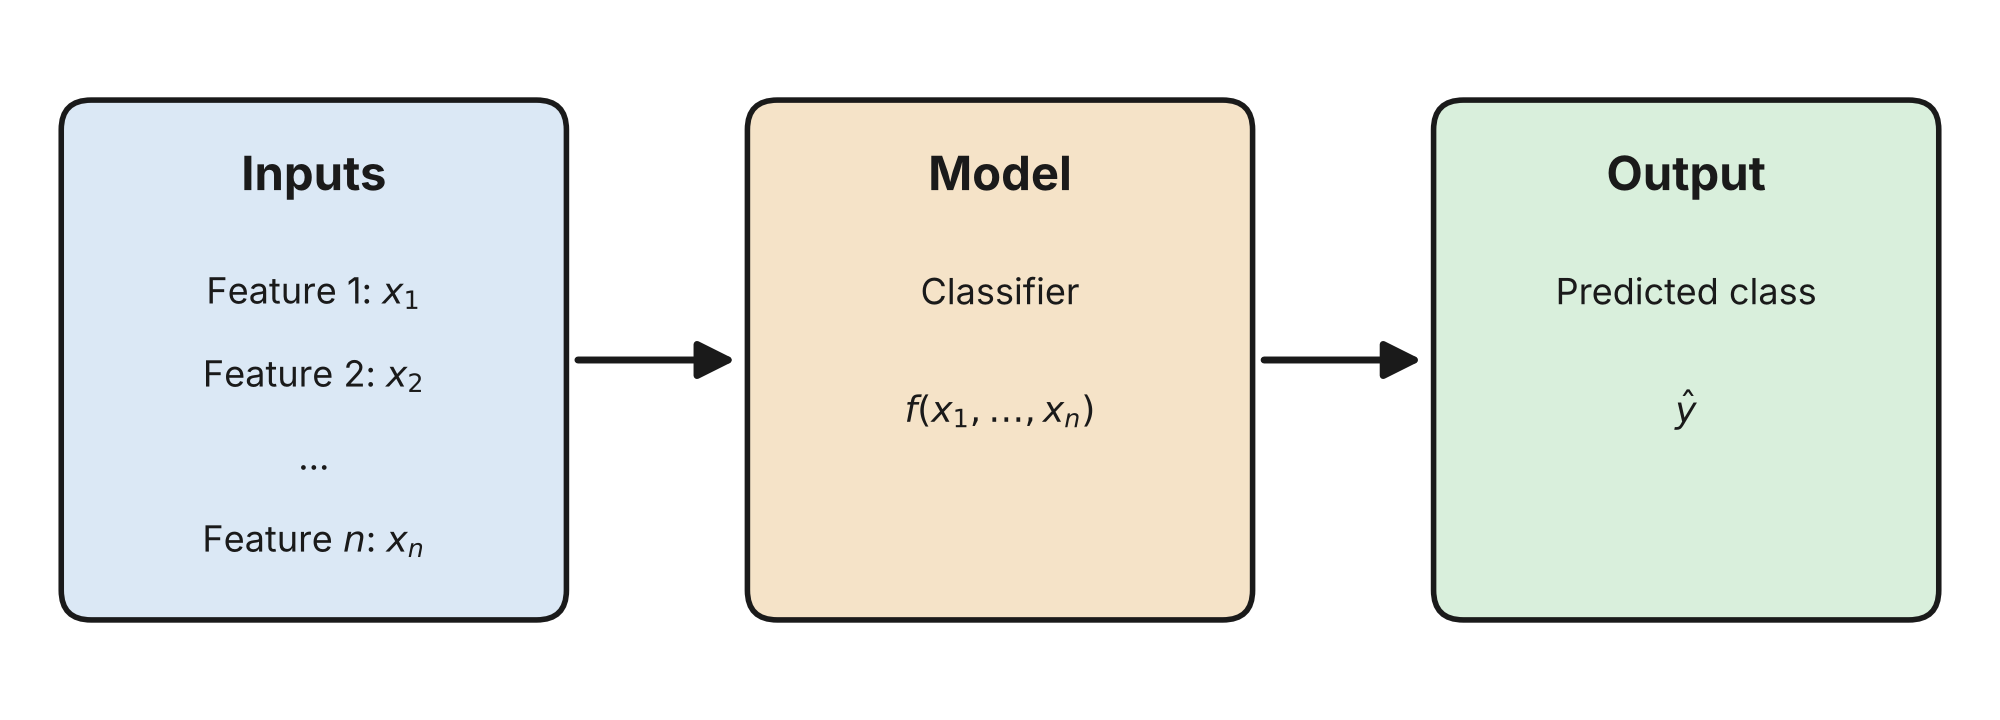
\includegraphics[
      width=0.8\linewidth,
      alt={Classifier diagram: input features feed a model block, which outputs a predicted class. Full description in Appendix B.}
    ]{images/classifier.png}
    \caption{Example Classifier Diagram (\hyperref[sec:classifier-desc]{\textbf{Extended Description}})}
    \label{fig:classifier}
\end{figure}
\returnanchor{anchor:classifier-return}

For a full, narrative-style description of the classifier diagram, see Appendix~\ref{sec:classifier-desc}.

\subsection{Decorative Images (Artifacts)}
Not every image carries information. Decorative elements such as borders, background textures, and section dividers should be marked as \emph{artifacts} with the \texttt{artifact} key instead of being given alt text. Screen readers then skip them, so users are not interrupted by descriptions like ``decorative line.''

The divider below is an artifact:
\begin{verbatim}
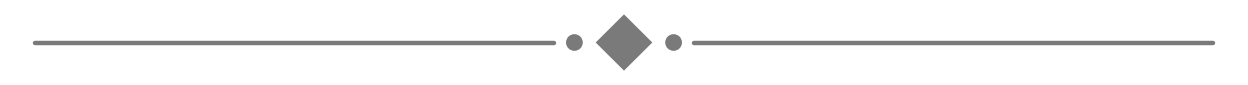
\includegraphics[width=0.6\linewidth, artifact]{images/section-divider.png}
\end{verbatim}

Use an artifact only when removing the image would lose no information. If an image conveys meaning, give it alt text instead.

\begin{center}
    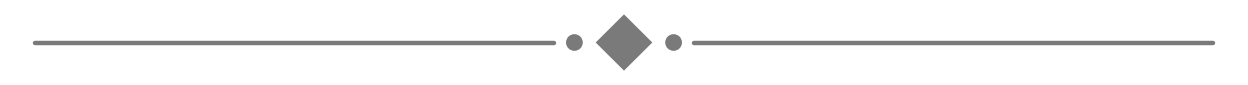
\includegraphics[width=0.6\linewidth, artifact]{images/section-divider.png}
\end{center}

%======================================================================%
% SECTION 6: LAYOUT
%======================================================================%
\section{Layout Practices: What to Avoid}
Avoid layout hacks like repeated \verb|\\| or \verb|\vspace|. Let LaTeX handle spacing so the reading order is preserved.

%======================================================================%
% SECTION 7: FINAL CHECK AND VALIDATION (CRITICAL)
%======================================================================%
\section{Final Check and Validation}
\label{sec:validation}

\subsection{PDF/UA-2 vs. Reality}
This document targets \textbf{PDF/UA-2} [3], [5]. Be aware of the limits of current tools:

\begin{itemize}
    \item \textbf{Institutional checkers:} Ally, Panorama, and the Adobe Acrobat accessibility checker do not support PDF 2.0 or PDF/UA-2 (vendor-confirmed). They may flag valid MathML or modern table structures as errors, for example reporting equations as missing alt text because they expect the older PDF/UA-1 approach. They may even score this document lower than a less accessible PDF/UA-1 file, so a low score from these tools does not mean the document is inaccessible.
    \item \textbf{PAC:} Fully supports PDF 1.7 documents only; PDF/UA-2 support is limited, with full support planned for a future release.
    \item \textbf{veraPDF:} Validates PDF/UA-2, but only the machine-verifiable rules [6]. Requirements that need human judgment, such as whether alt text is meaningful or reading order is logical, are outside any automated validator.
    \item \textbf{The real test:} Read the document with \textbf{NVDA + MathCAT}. If the headings, lists, tables, and equations are read and navigable, the content is accessible regardless of an automated score.
\end{itemize}

\subsection{Recommended Validation Steps}
\begin{enumerate}
    \item \textbf{Compile log:} Check the \texttt{check-tagging-status} report for incompatible packages, and look for warnings about unknown keys.
    \item \textbf{veraPDF:} Validate against the PDF/UA-2 profile.
    \item \textbf{Screen reader review:} Test with NVDA and MathCAT so headings, lists, tables, and equations are read correctly.
    \item \textbf{Reading order review:} Verify the logical order in Acrobat's Tags panel.
\end{enumerate}

%======================================================================%
% REFERENCES
%======================================================================%
\section{References}
\label{sec:references}

\begin{enumerate}
    \item U. Fischer and F. Mittelbach, ``News from the LaTeX Tagged PDF project: 2025,'' \emph{TUGboat}, vol. 46, no. 2, 2025.

    \item LaTeX Project Team, ``Using LaTeX to produce accessible PDF,'' \emph{LaTeX Tagging Project}. [Online]. Available: \url{https://tagging-project.latex-project.org/documentation/usage-instructions}

    \item ISO, ``Document management applications --- Electronic document file format enhancement for accessibility --- Part 2: Use of ISO 32000-2 (PDF/UA-2),'' ISO 14289-2:2024, Geneva, Switzerland, 2024.

    \item N. Soiffer, ``MathCAT: Math Capable Assistive Technology,'' \emph{GitHub Repository}. [Online]. Available: \url{https://github.com/NSoiffer/MathCAT}

    \item PDF Association, ``Well-Tagged PDF (WTPDF),'' \emph{PDF Association Technical Specification}, 2024.

    \item veraPDF Consortium, ``veraPDF: Industry Supported PDF/A and PDF/UA Validation.'' [Online]. Available: \url{https://verapdf.org}

    \item LaTeX Project Team, ``Tagging Status of LaTeX Packages and Classes.'' [Online]. Available: \url{https://latex3.github.io/tagging-project/tagging-status/}
\end{enumerate}

%======================================================================%
% CREDITS
%======================================================================%
\section{Credits}

Developed and maintained by Gerry Pedraza and Christine Roach, Engineering Studio for Advanced Instruction and Learning (eSAIL), Texas A\&M University.

Research and testing contributions: Osvaldo Misael Cortes, Lydia K.\ Harrison, and Vinayaka Madhukeshwar Hegde.

This work builds on the LaTeX Tagging Project by the LaTeX Project Team. Template repository: \url{https://github.com/gerrypedraza/accessibility}. Suggestions and problem reports are welcome as issues on the repository.

%======================================================================%
% APPENDIX: LONG DESCRIPTIONS
%======================================================================%
\appendix
% Appendix divider page: the section heading itself is set large and
% centered on its own page, so it is still tagged as a real heading.
% The redefinition of \section stays local to this group.
\clearpage
\vspace*{\fill}
\begingroup
\makeatletter
\renewcommand\section{\@startsection{section}{1}{\z@}{0pt}{2ex}%
  {\normalfont\Huge\bfseries\centering}}
\makeatother
\section{Appendix: Long Descriptions}
\endgroup
\begin{center}
\large Extended descriptions of the figures in this document.
\end{center}
\vspace*{\fill}
\clearpage

\subsection{Extended Description: Compressive Strength Chart}
\label{sec:data-presentation-desc}
\textbf{Purpose.} Fig.~\ref{fig:data-presentation} compares how strong five concrete mixes become as they cure. It shows which mix is strongest and how much strength each mix gains between an early test (7 days) and the standard design test (28 days). The values are illustrative, not measured data.

\textbf{Layout.} The figure is a grouped bar chart titled ``Compressive Strength of Five Concrete Mixes.'' The horizontal axis, labeled ``Concrete mix,'' lists five mixes from left to right: Mix A, Mix B, Mix C, Mix D, and Mix E. The vertical axis, labeled ``Compressive strength (MPa),'' runs from 0 to 100 megapascals, with tick marks and light gray horizontal gridlines every 20~MPa. Each mix has a pair of side-by-side bars. The left bar of each pair shows strength after 7 days of curing and is light blue with diagonal hatching. The right bar shows strength after 28 days and is solid dark blue. The pattern, not only the color, distinguishes the two series. A legend titled ``Curing age'' in the upper left identifies the two bar styles, and every bar has its exact value printed above it.

\textbf{Data.} The table lists every value in the chart, plus the gain from 7 to 28 days.

\medskip
\tagpdfsetup{table/header-rows=1}
\begin{tabular}{l c c c}
    \toprule
    \textbf{Mix} & \textbf{7 days (MPa)} & \textbf{28 days (MPa)} & \textbf{Gain (MPa)} \\
    \midrule
    Mix A & 42 & 62 & 20 \\
    Mix B & 48 & 70 & 22 \\
    Mix C & 55 & 81 & 26 \\
    Mix D & 51 & 76 & 25 \\
    Mix E & 39 & 58 & 19 \\
    \bottomrule
\end{tabular}

\medskip
\textbf{Trends and comparisons.}
\begin{itemize}
    \item Every mix is stronger at 28 days than at 7 days. The gains range from 19~MPa (Mix E) to 26~MPa (Mix C).
    \item The ranking is the same at both ages. From strongest to weakest: Mix C, Mix D, Mix B, Mix A, Mix E.
    \item Mix C is the strongest mix at both ages, with 55~MPa at 7 days and 81~MPa at 28 days. Mix D is close behind, with 51 and 76~MPa.
    \item Mix E is the weakest at both ages, with 39 and 58~MPa. At 28 days, Mix C is 23~MPa (about 40\%) stronger than Mix E.
    \item For every mix, the 7-day strength is about two-thirds (67 to 69\%) of the 28-day strength, so the 7-day test is a consistent early predictor of final strength.
    \item Averaged across all five mixes, strength rises from 47~MPa at 7 days to about 69~MPa at 28 days.
\end{itemize}


% \ref* prints the number without its own link, avoiding a link nested in a link
\hyperref[anchor:data-presentation-return]{\textbf{[Return to Figure~\ref*{fig:data-presentation} in main content]}}

\subsection{Extended Description: Classifier Diagram}
\label{sec:classifier-desc}
\textbf{Purpose.} Fig.~\ref{fig:classifier} shows the basic structure of a classifier: information flows from a set of input measurements, through a model, to a single predicted category. It is meant to convey the idea that a classifier is a function, not the details of any particular algorithm.

\textbf{Layout.} The diagram is read from left to right. It contains three rounded rectangular boxes of equal size, side by side, each with a bold title at the top. Two thick black arrows connect them: one from the first box to the second, and one from the second box to the third. The boxes have different light fill colors (blue, orange, and green), but the colors carry no meaning; the titles and arrows convey the structure.

\textbf{The three boxes, in reading order.}
\begin{enumerate}
    \item \textbf{Inputs} (left, light blue): a vertical list of the features describing one item to be classified. It reads ``Feature 1: $x_1$,'' ``Feature 2: $x_2$,'' then an ellipsis indicating that more features follow, and finally ``Feature $n$: $x_n$.'' There can be any number of features, $n$, such as the measurements of a sample or the attributes of a record.
    \item \textbf{Model} (center, light orange): the word ``Classifier,'' with the function $f(x_1, \ldots, x_n)$ written below it. The notation shows that the model takes all $n$ feature values together as its arguments. The arrow from Inputs into this box shows the features being passed to the model.
    \item \textbf{Output} (right, light green): the words ``Predicted class,'' with the symbol $\hat{y}$ (read ``y hat'') below them. The hat marks it as an estimate made by the model rather than a known true value. The arrow from Model into this box shows the model producing its prediction.
\end{enumerate}

\textbf{Main idea.} Reading the three boxes in order gives the relationship $\hat{y} = f(x_1, \ldots, x_n)$: a classifier maps many input features to one predicted category. For example, the features might be the measurements of a flower, and the predicted class its species.

\hyperref[anchor:classifier-return]{\textbf{[Return to Figure~\ref*{fig:classifier} in main content]}}

% End marker: confirms the whole document rendered. Readable text (not an
% artifact), so screen reader users also hear where the document ends.
\vspace{3\baselineskip}
\begin{center}
\textbf{[End of Document]}
\end{center}

\end{document}
